% Figure 4.1 (Session 4): the coefficients of a chain as one tensor and as a matrix product state.
% The image is rendered by figures/blender/s4_1_mps_chain.py; the coordinates of the labels come
% from figures/blender/out/mps_chain_anchors.tex. Compile with:
%   pdflatex mps_chain.tex ; result moves to ../mps_spin_chains/mps_chain.pdf
\documentclass[11pt,tikz,border=0pt]{standalone}
\usepackage{amsmath,amssymb,graphicx}
\usepackage{xcolor}
\definecolor{coursedark}{HTML}{1B2A4A}
\definecolor{costamber}{HTML}{B8620A}
\newlength{\figw}\setlength{\figw}{16.19cm}   % the text width of the notes (letter, 2.7 cm margins), so labels print at size

\begin{document}
\begin{tikzpicture}[lbl/.style={font=\small, text=coursedark}]
  \node[anchor=south west, inner sep=0pt] at (0,0)
    {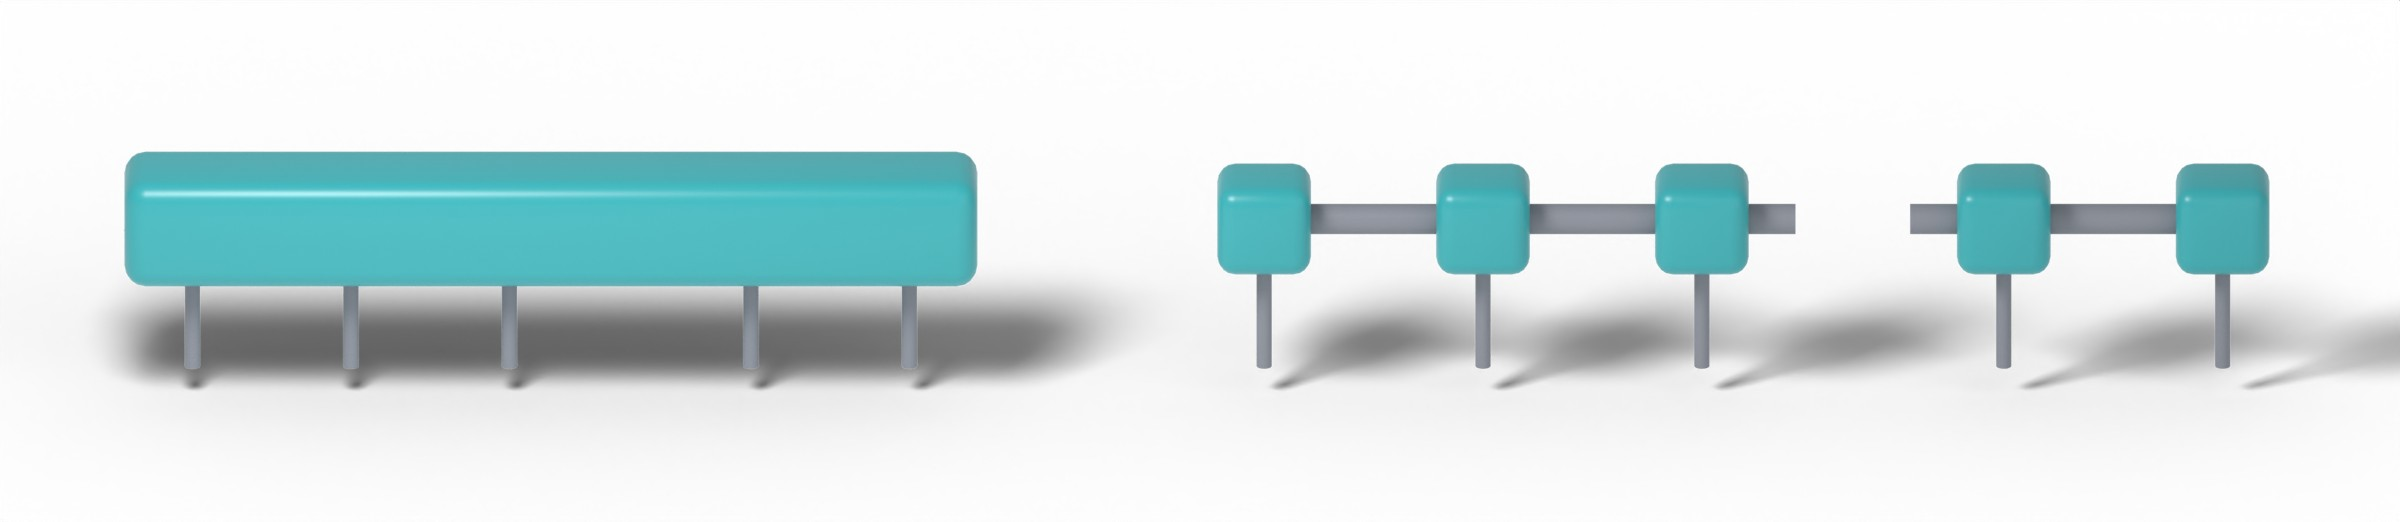
\includegraphics[width=\figw]{../blender/out/mps_chain.jpg}};
  %% written by figlib.py; x and y in units of the image width
\coordinate (as1) at (0.0802\figw,0.0534\figw);
\coordinate (as2) at (0.1462\figw,0.0534\figw);
\coordinate (as3) at (0.2123\figw,0.0534\figw);
\coordinate (asLm) at (0.3129\figw,0.0534\figw);
\coordinate (asL) at (0.3789\figw,0.0534\figw);
\coordinate (adots) at (0.2626\figw,0.0534\figw);
\coordinate (C) at (0.2296\figw,0.1583\figw);
\coordinate (a) at (0.0425\figw,0.2050\figw);
\coordinate (eq) at (0.4572\figw,0.1262\figw);
\coordinate (bs1) at (0.5267\figw,0.0534\figw);
\coordinate (M1) at (0.5267\figw,0.1525\figw);
\coordinate (bs2) at (0.6179\figw,0.0534\figw);
\coordinate (M2) at (0.6179\figw,0.1525\figw);
\coordinate (bs3) at (0.7091\figw,0.0534\figw);
\coordinate (M3) at (0.7091\figw,0.1525\figw);
\coordinate (bsLm) at (0.8349\figw,0.0534\figw);
\coordinate (MLm) at (0.8349\figw,0.1525\figw);
\coordinate (bsL) at (0.9261\figw,0.0534\figw);
\coordinate (ML) at (0.9261\figw,0.1525\figw);
\coordinate (chi0) at (0.5723\figw,0.1146\figw);
\coordinate (chi1) at (0.6635\figw,0.1146\figw);
\coordinate (bonddots) at (0.7720\figw,0.1262\figw);
\coordinate (chi3) at (0.8805\figw,0.1146\figw);
\coordinate (bdots) at (0.7720\figw,0.0534\figw);
\coordinate (b) at (0.4890\figw,0.2050\figw);

  \node[lbl, font=\normalsize, anchor=west] at (a) {(a)};
  \node[lbl, font=\normalsize, anchor=west] at (b) {(b)};
  \node[lbl, anchor=south] at (C) {$C(s_1,\ldots,s_L)$, $d^L$ numbers};
  \node[lbl, font=\large] at (eq) {$=$};
  \foreach \p in {a,b} {
    \node[lbl, anchor=north] at (\p s1) {$s_1$};
    \node[lbl, anchor=north] at (\p s2) {$s_2$};
    \node[lbl, anchor=north] at (\p s3) {$s_3$};
    \node[lbl, anchor=north] at (\p sLm) {$s_{L-1}$};
    \node[lbl, anchor=north] at (\p sL) {$s_L$};
    \node[lbl, anchor=north] at (\p dots) {$\cdots$};
  }
  \node[lbl] at (bonddots) {$\cdots$};
  \node[lbl, anchor=south] at (M1) {$M_1^{s_1}$};
  \node[lbl, anchor=south] at (M2) {$M_2^{s_2}$};
  \node[lbl, anchor=south] at (M3) {$M_3^{s_3}$};
  \node[lbl, anchor=south] at (MLm) {$M_{L-1}^{s_{L-1}}$};
  \node[lbl, anchor=south] at (ML) {$M_L^{s_L}$};
  \foreach \i in {0,1,3} \node[lbl, anchor=north] at (chi\i) {$\chi$};
\end{tikzpicture}
\end{document}
